\documentclass[letterpaper,twocolumn,openany,nodeprecatedcode]{dndbook}

% Use babel or polyglossia to automatically redefine macros for terms
% Armor Class, Level, etc...
% Default output is in English; captions are located in lib/dndstring-captions.sty.
% If no captions exist for a language, English will be used.
%1. To load a language with babel:
%	\usepackage[<lang>]{babel}
%2. To load a language with polyglossia:
%	\usepackage{polyglossia}
%	\setdefaultlanguage{<lang>}
\usepackage[english]{babel}
%\usepackage[italian]{babel}
% For further options (multilanguage documents, hypenations, language environments...)
% please refer to babel/polyglossia's documentation.

\usepackage[utf8]{inputenc}
\usepackage[singlelinecheck=false]{caption}
\usepackage{listings}
\usepackage{shortvrb}
\usepackage{stfloats}
\usepackage[english]{babel}
\usepackage[table]{xcolor} % for row colors
\usepackage{booktabs} % nicer horizontal lines
%\usepackage[compat=1.18]{tikz}
\usepackage{graphicx}


\captionsetup[table]{labelformat=empty,font={sf,sc,bf,},skip=0pt}

\MakeShortVerb{|}

\lstset{%
  basicstyle=\ttfamily,
  language=[LaTeX]{TeX},
  breaklines=true,
}

%\title{Blizzard in the Night \\
%\large 30 days of night-ish}
%\author{J.B.Dennison}
%\date{2025/07/18}

\begin{document}
\DndSetThemeColor[DmgLilac]

%-------------------------------------------------------
% FRONT MATTER
%-------------------------------------------------------
\title{Blizzard in the Night \\
\large A Dungeons \& Dragons 5e Adventure for Characters of Levels 1–5} 
\author{J.B. Dennison}
\maketitle

\begin{DndReadAloud}
A month of darkness descends upon the remote frontier town of Barrow. As the sun fails to rise, something ancient stirs in the night — and the townsfolk begin to vanish one by one.
\end{DndReadAloud}


\section{Adventure Summary}
\DndDropCapLine{T}he Longest Night is a survival horror adventure for 1st- to 5th-level characters.  
The heroes arrive in Barrow just as the sun sets for what should be a brief polar night — but when dawn never comes, panic sets in.  
As supplies dwindle and terror mounts, the party must protect the townsfolk, uncover the cause of the endless darkness, and confront the creatures that thrive within it. 
Designed for 3–5 sessions, this adventure blends investigation, social intrigue, and escalating horror, culminating in a desperate stand against an ancient evil feeding on fear and blood.

\frontmatter

\maketitle

\tableofcontents

\mainmatter%

%-------------------------------------------------------
% INTRODUCTION
%-------------------------------------------------------
\chapter{Introduction}


\subsection{Adventure Overview}

\DndDropCapLine{F}{ar to the north lies the remote mining town of Barrow}, perched at the edge of civilization where the sun sets for months at a time.  
Each winter, the people of Barrow prepare for the long night — stockpiling food, oil, and wood to endure weeks without sunlight.  
But this year, something is different.  

As the days grow shorter, strange omens spread through the region: animals fleeing south, faint whispers carried on the wind, and travelers who vanish along the frozen road.  
When the final sunset comes, it brings not only darkness — but hunger.  

\textit{The Longest Night} places adventurers in an isolated town trapped under unending nightfall.  
The heroes must investigate the cause of the perpetual darkness, protect Barrow’s dwindling survivors, and face the growing horrors that hunt in the cold.  
As paranoia spreads and trust erodes, the line between survivor and predator begins to blur.  

This adventure blends survival horror, mystery, and moral tension.  
Combat encounters grow deadlier as resources run scarce, and decisions made early in the adventure — who to trust, who to save — echo through its grim conclusion.

\subsection{Adventure Hooks}

Each hook provides a reason for the characters to travel to Barrow just before the sun sets for the long winter.  
Choose one or more based on the party’s background or campaign setting.

\begin{itemize}
    \item \textbf{The Supply Run.}  
    A trading company hires the characters to deliver a final shipment of supplies — food, coal, and lantern oil — before the polar night begins.  
    The contract includes payment upon return, giving the party every reason to depart quickly once the job is done.
    
    \item \textbf{Summons from the North.}  
    A letter from an old friend, relative, or mentor in Barrow begs for help investigating mysterious disappearances and “signs in the sky.”  
    When the heroes arrive, the messenger who sent it is nowhere to be found.
    
    \item \textbf{Frontier Opportunity.}  
    Rumors claim that the mining operation in Barrow struck a rich vein of silver before winter — and the heroes have come to stake their claim, find work, or escort an investor hoping to profit before the thaw.
    
    \item \textbf{A Holy Omen.}  
    Clergy or scholars believe Barrow’s extended darkness fulfills an ancient prophecy tied to celestial alignment.  
    The characters are sent to investigate — or prevent — the coming of a foretold “long night of blood.”
    
    \item \textbf{The Northern Road.}  
    The party is simply passing through Barrow on their way farther north, only to find the roads closing behind them as the first blizzard rolls in.
\end{itemize}
\subsection{Surviving the Icy Wastes}

The polar wilderness around Barrow is as deadly as the creatures that stalk it.  
Adventurers must contend with frigid temperatures, blinding storms, and dwindling resources.  
The Dungeon Master should remind players that even simple travel or rest carries risk in this environment.
\section{Surviving in the Icy Wastes}

Traveling through the tundra around \textbf{Barrow} is as dangerous as any monster lurking in the dark. The cold, the shifting terrain, and the relentless weather can turn even a short journey into a deadly trial. Characters traveling through this environment must contend with several recurring hazards.
% ENVIRONMENT TABKLE
%\begin{table*}[b]% TO MAKE TABLES FULL WITH PUT DnDTable Inside another table like this
\begin{DndTable}[]{XXX}
\textbf{Hazard} & \textbf{Check / Save} & \textbf{Effect on Failure} \\
\hline
Avalanche & Dex Save DC 15 & 10d10 bludgeoning, restrained under snow \\
Blizzard & Con Save DC 10 +1/hr & 1 level exhaustion from cold \\
Frigid Water & Con Save DC 12 & 1 level exhaustion, 1d6 cold dmg/min \\
Mountain Travel & Surv. DC 15 / Athl. DC 14 & Lost, falls, exhaustion at high altitude \\
Extreme Cold & Con Save DC 10/hr & 1 level exhaustion from exposure \\
\hline
\end{DndTable}
%\end{table*}[b]%

\subsection{Avalanche}

A sudden avalanche can bury travelers beneath tons of snow and ice.

\textbf{Trigger:} Loud noises (e.g., spells, combat) or unstable slopes may trigger an avalanche.  
\textbf{Detection:} A successful DC~15 Wisdom (Perception) check allows a character to hear the groaning snow just before it collapses.  
\textbf{Avoidance:} Creatures in the affected area must make a DC~15 Dexterity saving throw, taking 10d10 bludgeoning damage on a failure, or half as much on a success. Failed saves also leave creatures \textit{restrained} beneath the snow.  
\textbf{Escape:} A restrained creature can attempt a DC~20 Strength (Athletics) check each round to dig free or be rescued by an ally using an action.

\subsection{Blizzard}

Blizzards sweep across the tundra with howling winds and freezing sleet that obscure vision and sap warmth.

\textbf{Effects:}
\begin{itemize}
  \item Visibility reduced to 30 feet; beyond that range creatures are \textit{heavily obscured}.
  \item Ranged weapon attacks are made with \textit{disadvantage}.
  \item Open flames are extinguished unless protected.
\end{itemize}

Each hour of exposure requires a DC~10 Constitution saving throw, increasing by +1 for each additional hour. Failure results in one level of \textit{exhaustion}.  
A DC~15 Wisdom (Survival) check prevents the party from becoming lost in the storm.

\subsection{Frigid Waters and Thin Ice}

Crossing frozen rivers or lakes carries risk—thin ice can collapse beneath travelers.

\textbf{Detection:} A DC~13 Wisdom (Perception) check reveals thin or cracking ice.  
\textbf{Falling In:} A creature that falls through must succeed on a DC~12 Constitution saving throw or suffer one level of \textit{exhaustion} from shock.  
Each minute in frigid water, the creature must make a DC~10 Constitution saving throw or take 1d6 cold damage and gain one level of exhaustion.  
\textbf{Escape:} Climbing out requires a DC~10 Strength (Athletics) check (made with disadvantage unless aided).

\subsection{Mountain Travel}

The high ridges and ice-clad peaks near Barrow are treacherous and unpredictable.

\textbf{Navigation:} Each hour requires a DC~15 Wisdom (Survival) check to avoid losing the path.  
\textbf{Climbing:} Icy cliffs require a DC~14 Strength (Athletics) check. Failure by 5 or more causes a fall.  
\textbf{Falling:} Take 1d6 bludgeoning damage per 10 feet fallen; landing on ice adds +5 damage.  
\textbf{Altitude:} Time spent above 10{,}000 ft without acclimation imposes one level of exhaustion every 6 hours.

\subsection{Cold Weather Survival}

The region around Barrow is classified as \textit{extreme cold} (DMG p.~110).  
A creature exposed to temperatures below 0°F must succeed on a DC~10 Constitution saving throw each hour or gain one level of exhaustion.  
Characters wearing cold-weather gear (furs, cloaks, or a \textit{ring of warmth}) automatically succeed.  
Creatures naturally adapted to cold climates (such as goliaths, white dragons, or winter wolves) are immune to these effects.


\subsection{Character Secrets and Background Ties}

To intensify suspicion and personal stakes, each character may carry a secret known only to them and the Dungeon Master.  
These secrets can relate to the darkness, Barrow’s people, or the player’s own past.

Before play begins, the DM may present each player with one or more secret prompts to choose from or roll randomly.  
Some examples include:

\begin{itemize}
    \item You once lived in Barrow—and fled after something you did one winter night.  
    Someone here remembers you.
    \item You carry an heirloom symbol of an ancient faith. Its markings match those carved into the mine walls.
    \item You came north to escape a bounty or a curse that still follows you.  
    The endless night might awaken it.
    \item You secretly dream of a voice calling from the darkness.  
    Each day, it becomes harder to resist.
    \item You are hiding an infection, wound, or strange mark from the others.  
    You fear what it might mean.
\end{itemize}

\usetikzlibrary{shapes.geometric, arrows.meta, positioning}
\newpage	
\section{Chapter Overview}

% === D&D Adventure Flowchart ===
\begin{center}
\begin{tikzpicture}[
    chapter/.style={
        rectangle,
        rounded corners,
        draw=black!80,
        fill=blue!10,
        text width=16cm,
        align=center,
        font=\bfseries\small,
        minimum height=1.5cm,
        inner sep=10pt
    },
    arrow/.style={thick, -{Stealth[length=5pt,width=7pt]}, black!70},
    node distance=2.5cm
]

% --- Nodes ---
\node[chapter] (ch1) {
    \textbf{Chapter 1: Journey to Barrow}\\
    \textit{Level 1–3}\\[3pt]
    The heroes travel through icy wilderness toward the remote town of Barrow. 
    A deadly blizzard forces them to seek shelter. Strange tracks, frozen corpses, and 
    fearful travelers set an ominous tone.
};

\node[chapter, below=of ch1] (ch2) {
    \textbf{Chapter 2: Shadows in the Snow}\\
    \textit{Level 3–4}\\[3pt]
    Trapped by the storm, the party investigates mysterious disappearances. 
    Superstitions and red herrings abound—wolves, curses, and suspicious townsfolk—
    while subtle clues hint at a darker truth beneath the ice.
};

\node[chapter, below=of ch2] (ch3) {
    \textbf{Chapter 3: The Blood Beneath Barrow}\\
    \textit{Level 4–5}\\[3pt]
    The heroes uncover that ancient vampires dwell beneath the town. 
    They rally allies, bless weapons, and fortify Barrow for the coming siege. 
    Knowledge, faith, and preparation determine who will survive the long night.
};

\node[chapter, below=of ch3] (ch4) {
    \textbf{Chapter 4: The Night Siege of Barrow}\\
    \textit{Level 5–6}\\[3pt]
    When darkness falls, the vampires strike. 
    The final battle rages through the snow-covered streets and tunnels. 
    Choices made earlier—alliances, wards, and tactics—shape the fate of Barrow.
};

% --- Arrows ---
\draw[arrow] (ch1) -- (ch2);
\draw[arrow] (ch2) -- (ch3);
\draw[arrow] (ch3) -- (ch4);

\end{tikzpicture}
\end{center}
\chapter{The Call Before the Long Night}
\label{chap:the-call-before-the-long-night}

\section*{Background and Life in Ten-Towns}

The far north lies in half-light. The sun lays low above the horizon, and its brief glow fades to twilight before most can finish their morning chores. The Ten-Towns endure this cycle every year, their citizens hardened to the dark and cold. Yet this winter feels different—colder, longer, and hungrier.

Life in the Ten-Towns is harsh, but Bryn Shandar is one of the fiendliest and most comfortable there is here. Each settlement depends on trade, fishing, and mining, and all rely on Bryn Shandar as the hub for supplies and protection. The long winters demand cooperation: strangers are rare, and hospitality is sacred. Those who betray the trust of the towns find no welcome when the blizzards rise.

Physically Bryn Shandar stands out among the ten towns. Designed as atop a hill in a wide birth circle, with 30 foot tall walls and towns gates half that high.

\subsection{Cold Weather Gear}

Adventurers who venture north require proper equipment. Even within the wals of Bryn Shandar cold weather gear can prove a boon.A creature exposed to temperatures below 0°F must succeed on a DC~10 Constitution saving throw each hour or gain one level of exhaustion *unless they have cold weather clothing*.  
\begin{itemize}
  \item \textbf{Cold-weather clothing} (10 gp): A fur-lined coat, boots, mittens, and layers of wool and leather. Provides resistance to exhaustion from cold weather.
  \item \textbf{Snowshoes} (2 gp): Negates difficult terrain caused by deep snow.
  \item \textbf{Climbing gear and ice picks} (25 gp): Essential for frozen slopes and glacial ravines.
  \item \textbf{Sled and team of dogs} (50 gp): For carrying cargo or wounded companions.
\end{itemize}

Without such gear, exposure checks occur hourly (Constitution save DC 10, increasing by 1 each hour). Failure results in one level of exhaustion.

\subsection{Magic in Ten-Towns}

Arcane magic is regarded with wary respect in the Ten-Towns. Most folk trust only divine miracles—prayers to Auril for mercy, to Tempus for strength, or to Chauntea for food. Wizards and sorcerers are tolerated, but their talents often invite suspicion, especially during the long nights when strange lights dance in the sky.

Magical services are rare and expensive. Minor healing or weather wards might be offered by the local priest for a donation of 25–50 gp, but powerful spells are nearly unheard of.  
In Bryn Shandar, a few retired adventurers and scholars maintain small collections of scrolls, potions, and trinkets—useful, if one knows where to look.

\subsection{Fuel and Light}

The cold claims more lives than monsters. In Ten-Towns, warmth is survival. Firewood is precious, coal is rarer still, and whale oil is hoarded for the long dark. Torches burn quickly in the frigid wind; lanterns and magical light are invaluable.

Each settlement maintains a communal hearth that burns day and night. During blizzards, people gather there to share warmth and food—an unspoken rule among the townsfolk. Extinguishing a hearth-fire, intentionally or by neglect, is seen as a grave offense.

\section{Running This Chapter}

This is the starting town in the Long Night campaign. Each of your players should have a pre-designed hook to go to Barrow town. While there is a bit of \textit{kismet} involved with them all being at the inn for the cute meet as the caravanners yell out for any extra help for their travels north, this section is filled with choice. There are 10 quests in town that the characters may choose to pursue or not which will lend several boons or banes depending on how they lay out. Additionally, characters are free to make their own way north.

\subsection*{Pacing and Structure}

\begin{itemize}
    \item \textbf{Day 1: Arrival and Orientation} — Introduce Bryn Shandar, its people, and the common hall. Present the caravan master and announce the upcoming departure. Allow players to meet NPCs and learn about the town’s daily rhythms.
    \item \textbf{Day 2: Exploration and Side Quests} — Encourage characters to pursue personal hooks and optional quests. Use skill challenges (Persuasion, Investigation, Survival, Animal Handling) to resolve minor tasks. Introduce subtle foreshadowing of the northern hazards or the supernatural.
    \item \textbf{Day 3: Wrapping Up and Caravan Preparation} — Resolve remaining quests, provide any final clues or advantages, and have the caravan load. Allow PCs to negotiate for better gear, mounts, or provisions. End the day with a ritual, festival, or communal event to heighten stakes and morale.
\end{itemize}


\subsubsection{Transition to Chapter 2}

At the end of Day 3, the DM should gather the party at the town gates, ready to load the caravan. Describe the mounting blizzard, the sound of sled bells, and the tension of leaving civilization behind. This naturally transitions into Chapter 2: \textit{Into the Wastes}, where the first real hazards and mysteries of the journey unfold.

\section{Cold Open}
Before starting discuss with each of your players what is drawing them to Barrow town and how they ended up in Bryn Shandar on the way north. Discuss the possible hooks and secrets from the Introduction, they may already be apart of the supply run by Torvald by the time the campaign starts and you can have Torvald introduce them as he mentions the first few quests. Read the following scene and allow the characters to Introduce themselves. At level 1 they shouldn't have too much to say about their past but wizards may have studied somewhere, they may be from some town, they may even discuss the hook for why they're headed north.
\begin{DndReadAloud}
\DndDropCapLine{F}{rom the south,} travelers cross the tundra to Bryn Shandar, the largest of the Ten-Towns. Within its wooden palisade, the air smells of smoke, leather, and frost. The markets bustle as merchants hurry to make their final trades before the snow seals the passes. Lanterns of colored glass sway in the wind, glimmering like distant stars.
\\
The great common hall hums with life—merchants, trappers, mercenaries, and miners warming themselves by the fire. Amid the laughter and the clink of mugs, a broad-shouldered caravan master named \textbf{Torvald Halmar} stands atop a bench and shouts above the din:
    “Three days! That’s all before the north road closes! I need sled-drivers and guards for the Barrow run—last supply haul before the long night! Food, coal, and lamp oil, bound for the miners up north! Pay’s fair, but the road’s not kind. Who’s in?”
\\
    Most of the crowd disperses with no interest travelling further north during this part of the year, but each of you has your own reason traveling to Barrow town. The \textit{NUMBER OF PLAYERS} of you separately approach Torvald and when it becomes clear no one else will, he turns to you all and says:
    
    “Ah so there are a bit of brave hearts left in the city tell me about yourselves.”
\\
\end{DndReadAloud}
From here have Torvald ask the characters to help out with quests Barrows Ledger, A Meal for the Journey, and Lantern Festival.

\begin{DndReadAloud}
Torvald nods slowly as each of you speaks, his weathered face softening from its earlier bark.  

"A good mix of sense and steel, he mutters, wiping the foam his beard. The caravan will need both."

He hops down from the bench and waves you toward a round table near the hearth, spreading a map of the northern tundra across it.  
The parchment curls at the corners from heat and age, marked with dark ink lines tracing the road north.  

``We leave in three days,’’ Torvald says. ``But first, there’s business here in Bryn Shandar that needs sorting before we can move. Our clerk Elda’s misplaced the shipment ledger—don’t ask how—and we still need fresh provisions for the sled teams.’’  


He squints toward the frost-laced windows:

``And if you’ve the time, lend a hand with the Lantern Festival tomorrow night. Spirits are low, and a bit of light before the dark never hurt anyone.’’
He rolls up the map, thumps it against his shoulder, and grins.  
``Now you're free to sit on your arses for three days and just meet me at the city gates, but you help me with those two, and I’ll make sure your names are carved in every toast between here and Barrow.’’

The fire crackles. Outside, the wind howls against the shutters, a lonely reminder of the cold road waiting beyond the walls. For now, though, the hall feels warm and alive—a small haven before the long night ahead.

\end{DndReadAloud}
\begin{DndMonster}{Torvald Halmar}
\DndMonsterType{Medium humanoid (dwarf), neutral good}

\DndMonsterBasics[
armor-class = {13 (leather armor)},
hit-points  = {45 (6d8 + 18)},
speed       = {25 ft.}
]

\DndMonsterAbilityScores[
str = 14,
dex = 12,
con = 16,
int = 11,
wis = 14,
cha = 13
]

\DndMonsterDetails[
skills = {Animal Handling +4, Perception +4, Survival +6, Persuasion +3},
senses = {darkvision 60 ft., passive Perception 14},
languages = {Common, Dwarvish},
challenge = {1 (200 XP)},
]

\DndMonsterAction{Keen Survivalist}
Torvald has advantage on Wisdom (Survival) checks made to navigate icy or mountainous terrain, and on checks to prevent getting lost in snowstorms.

\DndMonsterSection{Actions}

\DndMonsterAction{Multiattack}
Torvald makes two melee or ranged attacks.

\DndMonsterAction{Handaxe}
\textit{Melee Weapon Attack:} +4 to hit, reach 5 ft., one target. \textit{Hit:} 6 (1d8 + 2) slashing damage.

\DndMonsterAction{Light Crossbow}
\textit{Ranged Weapon Attack:} +3 to hit, range 80/320 ft., one target. \textit{Hit:} 5 (1d8 + 1) piercing damage.

\DndMonsterSection{Personality}
Torvald Halmar is a broad-shouldered dwarf with a braided beard streaked by frost and a laugh that could thaw ice.  
A lifelong caravanner, he’s known along the northern routes as a fair dealer and relentless optimist—until the weather turns.  
He believes no one conquers the tundra, only survives it by respecting her moods.

\DndMonsterSection{Roleplaying Torvald}
Torvald calls everyone “friend” or “traveler” until they prove otherwise. He values hard work, good ale, and well-trained sled beasts.  
When speaking, he gestures with whatever mug or tool is in hand, often punctuating his sentences with a hearty “Hah!”  
He distrusts wizards (“Book-folk freeze faster than ink in a gale”) but secretly keeps a charm of Moradin under his furs.  
If the players help him with his errands, he quickly adopts them as his “road-kin,” and later defends them fiercely when danger comes to Barrow.
\end{DndMonster}
\section{Quests in Bryn Shandar}

Characters have three in-game days before the caravan departs. During this time, they can explore the town, prepare for the journey, and build connections. Completing quests can grant useful allies, discounts, or supplies for the road north. Three quests are gained right after approaching Torvald in the tavern including Barrow's Ledger, A Meal for the Journey, and Lanter Festival. 

\begin{table*}[h!]
\begin{DndTable}[]{XXX}
\textbf{Quest Name} & \textbf{Description} & \textbf{Reward / Effect} \\
\hline
A Wolf for a Sled & Requisition a trained sled team or dire wolf from the kennels. & Mounts or sled for faster travel. \\
Barrow's Ledger & Assist a harried clerk tallying Barrow’s overdue accounts. & Learn about the town’s mining troubles. \\
Lantern Festival & Help set up Bryn Shandar’s farewell celebration before winter’s deep. & Advantage on social checks with townsfolk. \\
A Meal for the Journey & Hunt or fish to provide fresh food for the caravan. & Extra rations and goodwill from Torvald. \\
Snowbound Stranger & Aid a mysterious traveler snowed in outside the gates. & Gain a helpful NPC ally or clue about Barrow. \\
Frozen Forge & Help the blacksmith repair frozen hinges and wagon axles. & Discount on weapons or metal gear. \\
Temple Offerings & Deliver coal to the shrine of Tempus before the first blizzard. & Blessing granting +1 on saving throws vs cold. \\
Trade Troubles & Mediate a dispute between rival merchants. & Favor from Bryn Shandar’s council. \\
Message from the South & Deliver a late letter to the caravan office—addressed to “Barrow Overseer.” & Early hint of the mystery in Barrow. \\
The Lost Dog & Find a merchant’s runaway sled dog before nightfall. & Gratitude and animal supplies (oil, furs). \\
\hline
\end{DndTable}
\end{table*}
%----------Quest 1------------------

\section{Barrow's Ledger}

\subsection{Quest Summary}
The characters are pointed toward this quest by Torvald mentioning Elda by name. While Elda is embarrassed and will insist she doesn't need any help a bit of investigation will allow players to discover that Elda, the well-meaning but often tipsy town clerk, lost it in a “friendly” game of snow dice.  
While she's willing to pay to return the items, her opponents were not traders as she thought, but \textit{three kobolds in a trench coat} posing as a single “distinguished merchant” named \emph{Sir Tallscale}.  
Unless the adventurers recover the ledger—and the missing crates of lamp oil wagered in the same game—the caravan cannot depart.

\subsection{Getting the Quest}
After initial discussions with Torvald the players simply need to inquire about Elda
In the warmth of the common hall, Torvald the caravan master slams a mittened fist onto a supply crate. 
\begin{DndReadAloud}
    
``The last thing we need before heading north is missing paperwork!'' he growls.  
Beside him, a red-cheeked woman in too many scarves—Elda, the town clerk—winces and tries to hide behind her mug of ale.  
``It’s just a small mix-up,'' she insists. ``The... merchants seemed reputable! Very tall, all three—uh, one—of them!’’  
Torvald sighs. ``Please, for the love of Auril, find those ‘merchants’ before I freeze solid waiting for a signature.’’
\end{DndReadAloud}
\begin{figure}[h!] % [h!] suggests "here, if possible, force it"
        \centering
        \includegraphics[width=\linewidth]{Elda.png}
        \caption{Elda the Gnome}
        \label{fig:EldaTheGnome} % For referencing the figure later with \ref{fig:myimage}
\end{figure}

\subsection*{Running the Quest}
\textbf{Finding the Kobolds.}  
A DC~12 Investigation check (or asking around the market) reveals tracks leading to an abandoned storage barn on the edge of Bryn Shandar.  
Inside, the kobolds are arguing about who gets to wear the top hat next. If the players knock or are discovered before hand they must pass a DC Int 5 check or they will be fooled by the disguise.

\begin{DndSidebar}[float=!b]{Role Playing the Kobolds}
The trio—Snik, Drup, and Varka—are not malicious, merely opportunistic.  
They planned to sell the lamp oil to buy enough meat pies to last the winter.  
If the characters approach peacefully, the kobolds can be convinced to return the goods in exchange for:
\begin{itemize}
  \item A single hot meal,
  \item Promise of a legitimate delivery job with the caravan, or
  \item 5~gp for “dignity purposes.”
\end{itemize}
If talks fail, the kobolds attempt to bluff their way out, tripping over each other as the trench coat collapses in a heap of scaly panic.

\end{DndSidebar}

\textbf{Combat (Optional).}  
If the party attacks or threatens violence, treat the encounter as \textbf{3 kobolds (MM~p.~195)}.  
Fighting ends once one kobold is knocked out; the others immediately surrender, dramatically pleading for mercy “on behalf of Sir Tallscale.”
\textbf{Success.}  
The characters return the ledger and supplies to Torvald, earning warm thanks and a modest payment of \textbf{25~gp total}.  
Elda adds their names to the caravan roster, ensuring a smoother departure.  
Morale among the merchants improves, granting the party \textbf{advantage on Persuasion checks with caravan members} during Chapter~2.
\subsection*{Outcomes and Rewards}

\textbf{Failure or Delay.}  
If the players never recover the ledger, Torvald’s the caravan leaves short on supplies; future travel checks suffer a --1 penalty until they resupply. Players must use their own rations during Chapter 2 and make DC 10 Con save each night or gain 1 level of exhaustion from exposure during the travel.

\subsection*{Town Changes}
After this quest, the kobolds become semi-official helpers in town—seen awkwardly sweeping snow or trying to sell “authentic Bryn Shandar souvenirs” (rocks with faces drawn on them).  
Their antics can provide comic relief or rumors for later chapters.


\clearpage % Finish any text before the image
\begin{figure}[p] % 'p' = put on its own page
    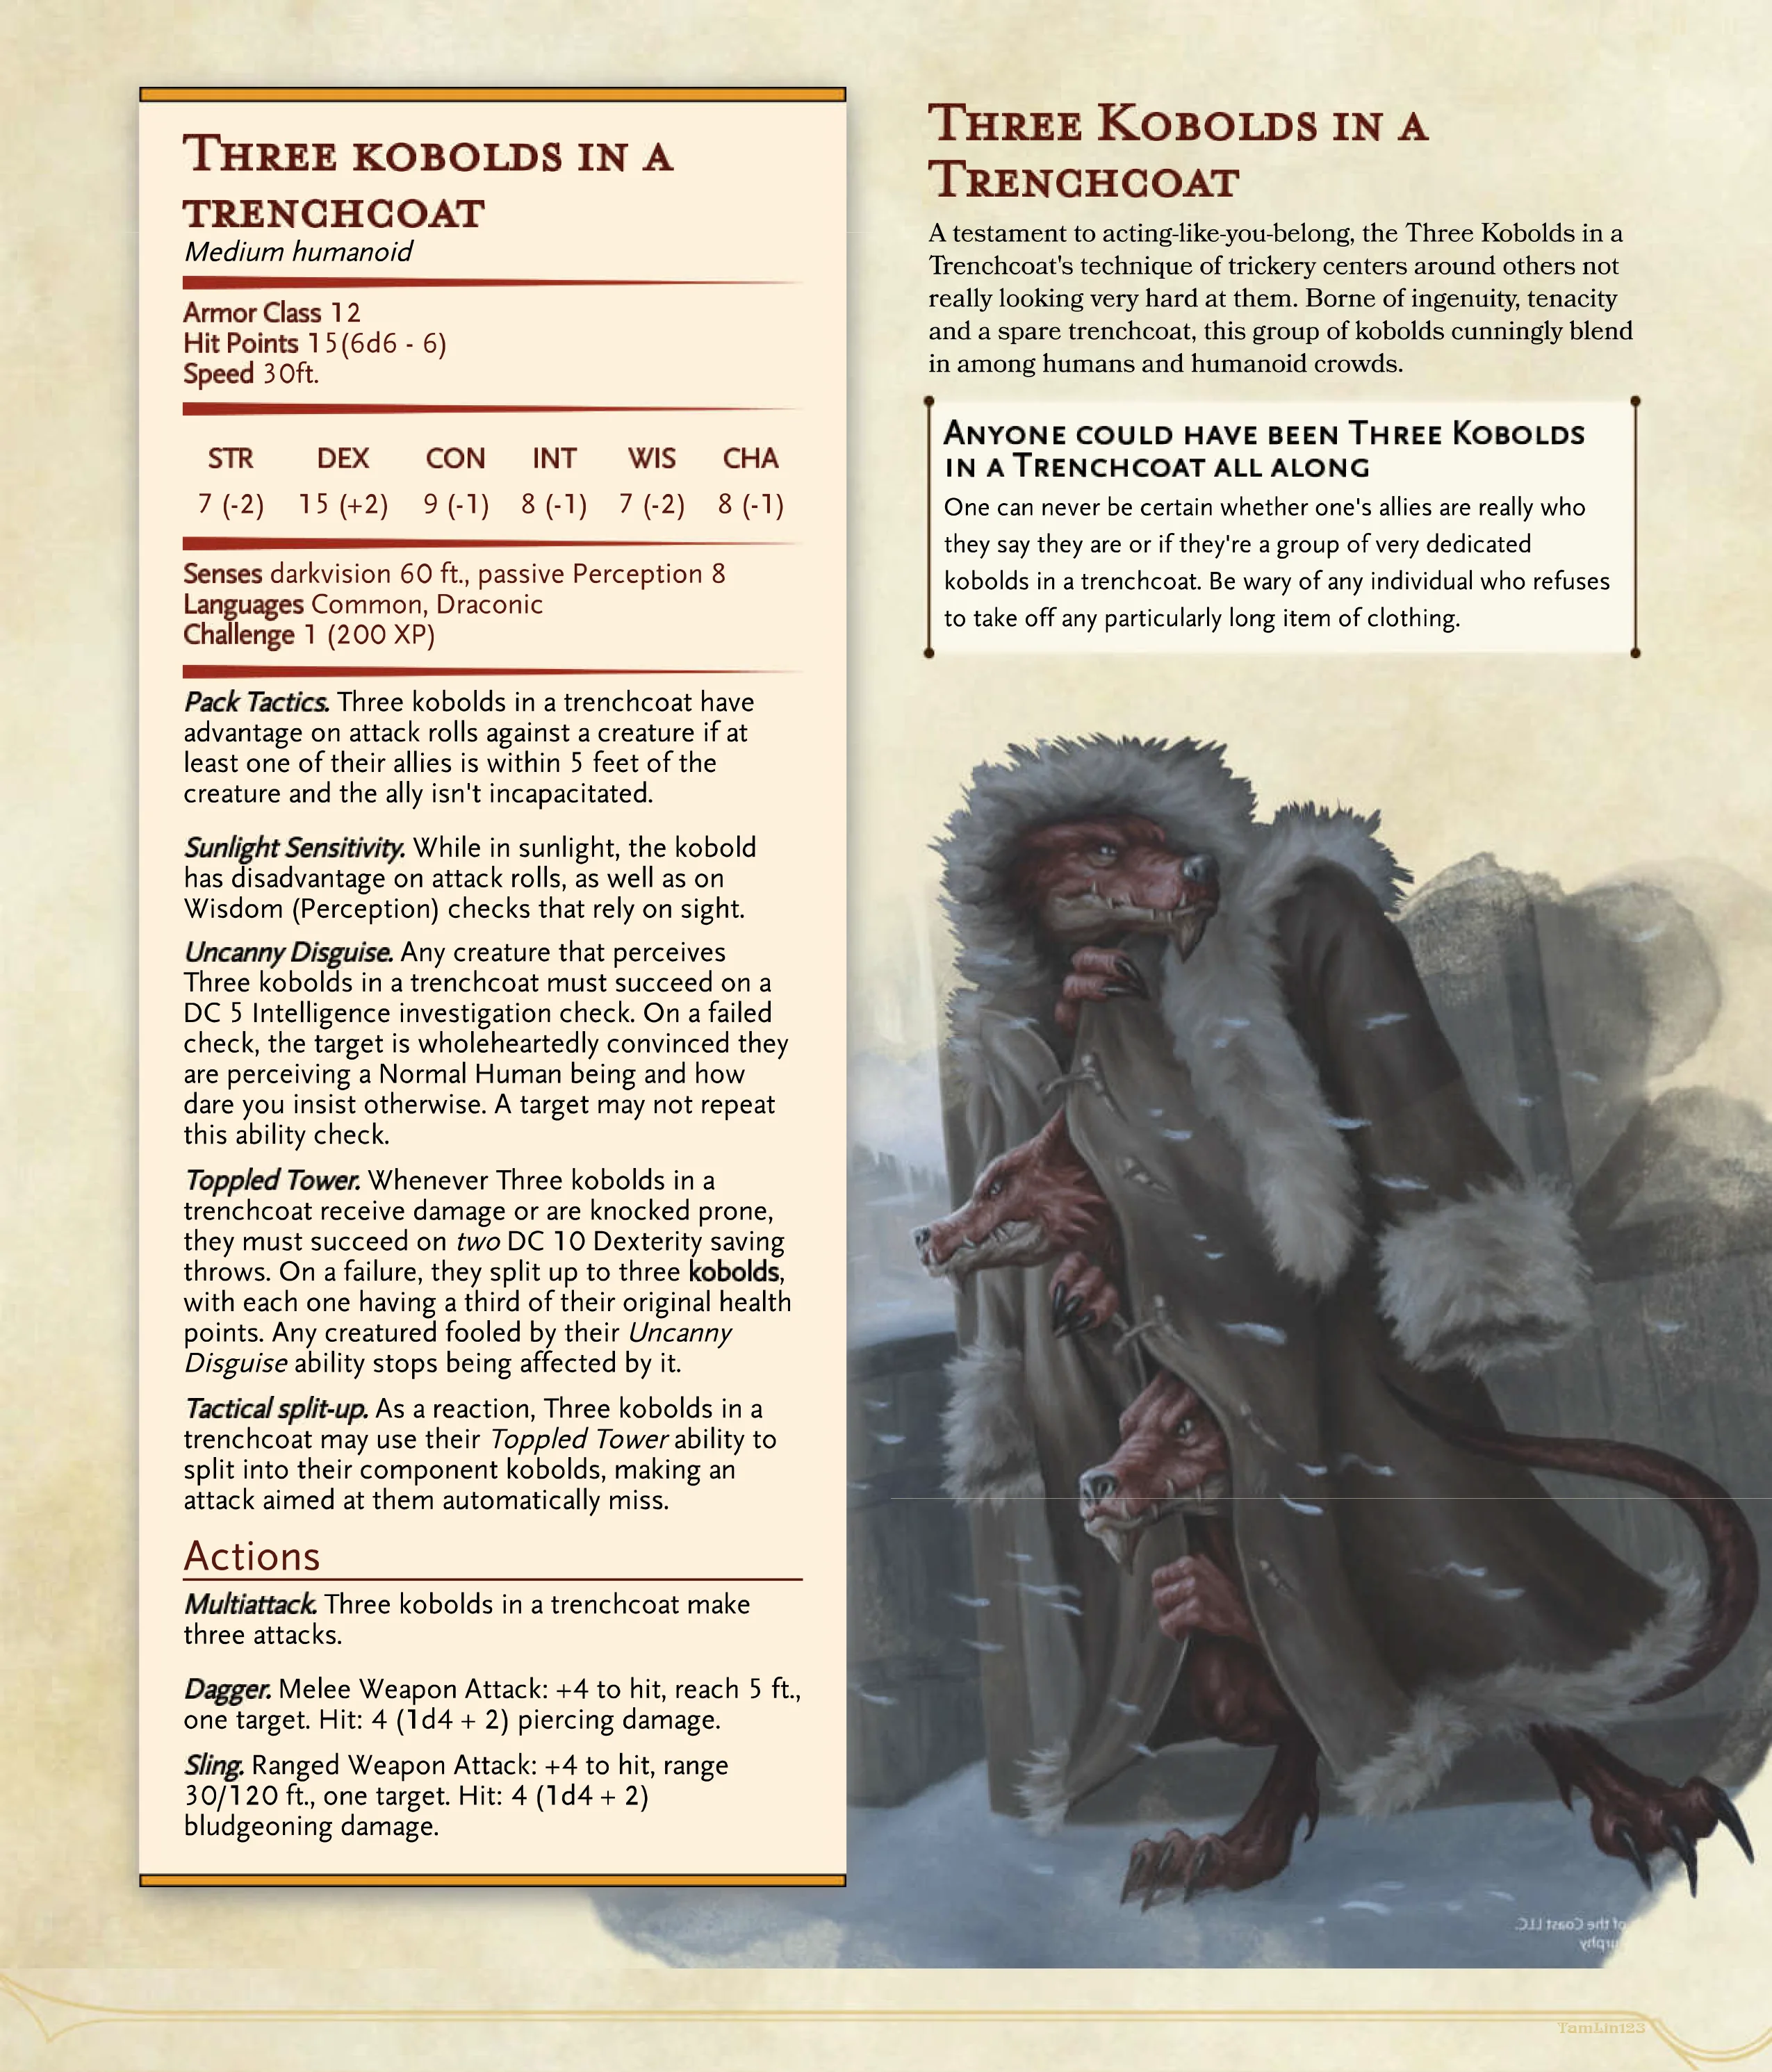
\includegraphics[width=1.15\textwidth,
    keepaspectratio]{Threekobolds.jpg}
    
\end{figure}
\clearpage % Start fresh text on the next page

%----------Quest 2------------------
\section{A Meal for the Journey}
\subsection{Quest Summary}
The caravan is nearly ready to depart, but a critical problem arises — the sleds are missing their provisions! 
Elda the caravan clerk miscounted the rations, and the butcher’s winter stock has already been sold. 
Without food, the northward journey will fail before it begins.

The party must find a way to secure enough food for the caravan within three days — by trade, hunt, persuasion, or ingenuity. 

\subsection{Getting the Quest}
After the initial gathering in the common hall, Torvald leans toward the adventurers with a weary sigh.

\begin{DndReadAloud}
\DndDropCapLine{B}{last it all,} we’ve sleds and oil enough to reach Barrow twice over, but nary a scrap to eat along the way.  
Elda miscounted the smoked trout barrels, and Skerren the butcher says he’s sold the rest to some bard troupe.  
If we leave hungry, we won’t make it past Lonelywood.  
Could you help me find us a meal fit for the road?
\end{DndReadAloud}

\subsection*{Running the Quest}
\textbf{Objective:} Gather a week’s worth of preserved food for the caravan before departure.  
Players can achieve this goal through several approaches — diplomacy, trade, or fieldwork.  
Encourage creativity and let success or failure shape how the caravan fares later in Chapter~2.

\subsubsection{ Convince Skerren the Butcher.}
\textit{Location: Skerren’s Smokehouse, Market District.}  
Skerren is a gruff, lonely man who has already sold the last shipment of smoked knucklehead trout to a bard troupe staying at the inn.

A DC~13 Persuasion check (or a favor such as helping with his festival preparations) convinces him to part with his personal reserve.  
Alternatively, an Insight check (DC~12) reveals that he simply wants some company and help hauling supplies.  
Earning his goodwill provides enough meat for the journey.

\subsubsection{2. Hunt or Fish for Fresh Provisions.}
Characters can venture onto the tundra to ice-fish or trap snow hares. When the characters venture beyond the walls of Bryn Shandar to hunt or fish, roll on the table below once every 2 hours spent in the wild.   

A DC~12 Survival check locates a good spot, followed by DC~11 Stealth or Nature to catch prey.  
They may encounter a friendly frost druid or awakened snow fox who teases them about “stealing from her pantry,” offering a few enchanted herbs as a peace offering if treated kindly.


\begin{DndTable}[header=Tundra Hunting Encounters]{1 X}
\textbf{d8} & \textbf{Encounter / Event} \\ \hline
1 & \textbf{Frozen Silence.} The wind dies completely. A DC~10 Perception check reveals strange shapes under the snow — half-buried fishing huts from years past. Searching them yields 1d4 preserved rations and a broken spear. \\ 
2 & \textbf{Snow Hare Tracks.} Fresh prints wind through the drifts. A DC~11 Survival check allows the party to catch 1d4 hares without incident. Failure draws the attention of a hungry fox or raven swarm. \\
3 & \textbf{Knucklehead Trout.} The ice near a frozen lake is thick but brittle. A DC~12 Survival check allows safe fishing for 1d4 trout. On a failed check, the ice cracks and one character must succeed on a DC~12 Dexterity save or fall into frigid water (see \textit{Frigid Water} hazard). \\
4 & \textbf{Hungry Wolf Pack.} 1d4 wolves (MM~p.~341) emerge from the snowdrifts, circling cautiously. They attack only if cornered or provoked. A DC~13 Animal Handling check can drive them off or allow the party to take a single injured wolf pup back to town. \\
5 & \textbf{The Frost Druid.} A cheerful frost druid named \textbf{Ysra Snowborn} (use druid stats, MM~p.~346) scolds the party for “stealing her hares.” If treated kindly, she gives the group a sprig of mistle toe which will create up to 10 Goodberries. \\
6 & \textbf{The Frozen Moose.} The party discovers a half-buried moose carcass. A DC~13 Nature or Medicine check determines it died of cold rather than predators. Carving it provides 1d6 rations but attracts scavengers (DC~12 Perception to notice them before attack). \\
7 & \textbf{Awakened Snow Fox.} A small white fox with intelligent eyes observes the party. It speaks telepathically, offering a “trade”: a few enchanted berries in exchange for a story or a joke. If amused, it gives the party 1d4 berries that restore 1 hit point each when eaten. \\
8 & \textbf{Whiteout.} A sudden blizzard sweeps over the tundra. All Survival checks for navigation or hunting are made at disadvantage until the party finds shelter or returns to town. Anyone left outside must succeed on a DC~10 Constitution saving throw or gain one level of exhaustion. \\
\hline
\end{DndTable}

\textit{Optional Flavor:}  
Roll with advantage if the players have previously befriended local trappers or gathered rumors in town.  
Failure to prepare cold-weather gear before venturing out results in disadvantage on all checks during the encounter.

\subsubsection{3. Cook with What You’ve Got.}
If all else fails, Elda panics and pulls together oats, lamp oil, and pickled radishes, insisting “it’s all about balance!”  
The party can attempt to make travel cakes using DC~10 Survival or Sleight of Hand checks to prepare them, and DC~12 Performance to make them seem edible.  
Success results in “Elda’s Ever-Oily Travel Cakes,” good for one meal per person — barely.

\paragraph{4. Negotiate with the Bard Troupe.}
The three half-elf performers staying at the inn will trade their smoked stock for amusement or favors.  
A DC~13 Performance or Deception check wins them over with a song, story, or clever bargain.  
A failed attempt offends them — they eat the rations in protest.

\begin{DndSidebar}[float=!b]{Flavorful Roleplay}
Lean into the humor and heart of this quest — Skerren may complain endlessly about “southern appetites,” 
Elda may try to sample raw lamp oil “for texture,” and the bard troupe can improvise verses mocking the party’s culinary attempts.  
These moments build warmth and personality in the frozen world of Ten-Towns.
\end{DndSidebar}

\subsection*{Outcomes and Rewards}

\textbf{Success.}  
The caravan departs well-stocked and grateful.  
Torvald thanks the heroes publicly, offering a reward of \textbf{25~gp total} and ensuring hearty meals on the road.  
The party gains \textbf{advantage on Constitution saving throws} against exhaustion during travel in Chapter~2.

\textbf{Partial Success.}  
If the party finds only partial or poor-quality provisions, the caravan remains uneasy.  
All Persuasion checks with caravan members suffer disadvantage until morale improves.

\textbf{Failure or Delay.}  
If no food is secured, the caravan must rely on player rations.  
During Chapter~2, all travel checks increase in DC by 1, and each night without food forces a DC~10 Constitution saving throw or gain one level of exhaustion.

\subsection*{Town Changes}
Following this quest, Elda proudly sells “Ever-Oily Travel Cakes” at the market during the Lantern Festival, claiming they’re “Bryn Shandar’s newest delicacy.”  
Skerren, impressed or horrified, becomes a recurring town contact — his smokehouse serving as a hub for gossip and future side quests.

\chapter{Two}
%-----------------------------------
\DndDropCapLine{T}{his package is designed to aid you in} writing beautifully typeset documents for the fifth edition of the world's greatest roleplaying game. It starts by adjusting the section formatting from the defaults in \LaTeX{} to something a bit more familiar to the reader. The chapter formatting is displayed above.

\section{Section}
Sections break up chapters into large groups of associated text.

\subsection{Subsection}
Subsections further break down the information for the reader.

\subsubsection{Subsubsection}
Subsubsections are the furthest division of text that still have a block header. Below this level, headers are displayed inline.

\paragraph{Paragraph}
The paragraph format is seldom used in the core books, but is available if you prefer it to the ``normal'' style.

\subparagraph{Subparagraph}
The subparagraph format with the paragraph indent is likely going to be more familiar to the reader.

\section{Special Sections}
The module also includes functions to aid in the proper typesetting of multi-line section headers: |\DndFeatHeader| for feats, |\DndItemHeader| magic items and traps, and |\DndSpellHeader| for spells.

\DndFeatHeader{Typesetting Savant}[Prerequisite: \LaTeX{} distribution]
You have acquired a package which aids in typesetting source material for one of your favorite games. You have advantage on Intelligence checks to typeset new content. On a failed check, you can ask questions online at the package's website.

\DndItemHeader{Foo's Quill}{Wondrous item, rare}
This quill has 3 charges. While holding it, you can use an action to expend 1 of its charges. The quill leaps from your hand and writes a contract applicable to your situation.

The quill regains 1d3 expended charges daily at dawn.

\DndSpellHeader%
  {Beautiful Typesetting}
  {4th-level illusion}
  {1 action}
  {5 feet}
  {S, M (ink and parchment, which the spell consumes)}
  {Until dispelled}
You are able to transform a written message of any length into a beautiful scroll. All creatures within range that can see the scroll must make a wisdom saving throw or be charmed by you until the spell ends.

While the creature is charmed by you, they cannot take their eyes off the scroll and cannot willingly move away from the scroll. Also, the targets can make a wisdom saving throw at the end of each of their turns. On a success, they are no longer charmed.

\section{Map Regions}
The map region functions |\DndArea| and |\DndSubArea| provide automatic numbering of areas.

\DndArea{Village of Hommlet}
This is the village of hommlet.

\DndSubArea{Inn of the Welcome Wench}
Inside the village is the inn of the Welcome Wench.

\DndSubArea{Blacksmith's Forge}
There's a blacksmith in town, too.

\DndArea{Foo's Castle}
This is foo's home, a hovel of mud and sticks.

\DndSubArea{Moat}
This ditch has a board spanning it.

\DndSubArea{Entrance}
A five-foot hole reveals the dirt floor illuminated by a hole in the roof.

\chapter{Text Boxes}

The module has three environments for setting text apart so that it is drawn to the reader's attention. |DndReadAloud| is used for text that a game master would read aloud.

\begin{DndReadAloud}
  As you approach this module you get a sense that the blood and tears of many generations went into its making. A warm feeling welcomes you as you type your first words.
\end{DndReadAloud}

\section{As an Aside}
The other two environments are the |DndComment| and the |DndSidebar|. The |DndComment| is breakable and can safely be used inline in the text.

\begin{DndComment}{This Is a Comment Box!}
  A |DndComment| is a box for minimal highlighting of text. It lacks the ornamentation of |DndSidebar|, but it can handle being broken over a column.
\end{DndComment}

The |DndSidebar| is not breakable and is best used floated toward a page corner as it is below.

\begin{DndSidebar}[float=!b]{Behold the DndSidebar!}
  The |DndSidebar| is used as a sidebar. It does not break over columns and is best used with a figure environment to float it to one corner of the page where the surrounding text can then flow around it.
\end{DndSidebar}

\section{Tables}
The |DndTable| colors the even rows and is set to the width of a line by default.

\begin{DndTable}[header=Nice Table]{XX}
    \textbf{Table head}  & \textbf{Table head} \\
    Some value  & Some value \\
    Some value  & Some value \\
    Some value  & Some value
\end{DndTable}

\chapter{Monsters and NPCs}

% Monster stat block
\begin{DndMonster}[float*=b,width=\textwidth + 8pt]{Monster Foo}
  \begin{multicols}{2}
    \DndMonsterType{Medium aberration (metasyntactic variable), neutral evil}

    % If you want to use commas in the key values, enclose the values in braces.
    \DndMonsterBasics[
        armor-class = {9 (12 with \emph{mage armor})},
        hit-points  = {\DndDice{3d8 + 3}},
        speed       = {30 ft., fly 30 ft.},
      ]

    \DndMonsterAbilityScores[
        str = 12,
        dex = 8,
        con = 13,
        int = 10,
        wis = 14,
        cha = 15,
      ]

    \DndMonsterDetails[
        %saving-throws = {Str +0, Dex +0, Con +0, Int +0, Wis +0, Cha +0},
        %skills = {Acrobatics +0, Animal Handling +0, Arcana +0, Athletics +0, Deception +0, History +0, Insight +0, Intimidation +0, Investigation +0, Medicine +0, Nature +0, Perception +0, Performance +0, Persuasion +0, Religion +0, Sleight of Hand +0, Stealth +0, Survival +0},
        %damage-vulnerabilities = {cold},
        %damage-resistances = {bludgeoning, piercing, and slashing from nonmagical attacks},
        %damage-immunities = {poison},
        %condition-immunities = {poisoned},
        senses = {darkvision 60 ft., passive Perception 10},
        languages = {Common, Goblin, Undercommon},
        challenge = 1,
      ]
    % Traits
    \DndMonsterAction{Innate Spellcasting}
    Foo's spellcasting ability is Charisma (spell save DC 12, +4 to hit with spell attacks). It can innately cast the following spells, requiring no material components:
    \begin{DndMonsterSpells}
      \DndInnateSpellLevel{misty step}
      \DndInnateSpellLevel[3]{fog cloud, rope trick}
      \DndInnateSpellLevel[1]{identify}
    \end{DndMonsterSpells}

    \DndMonsterAction{Spellcasting}
    Foo is a 2nd-level spellcaster. Its spellcasting ability is Charisma (spell save DC 12, +4 to hit with spell attacks). It has the following sorcerer spells prepared:
    \begin{DndMonsterSpells}
      \DndMonsterSpellLevel{blade ward, fire bolt, light, shocking grasp}
      \DndMonsterSpellLevel[1][3]{burning hands, mage armor, shield}
    \end{DndMonsterSpells}

    \DndMonsterSection{Actions}
    \DndMonsterAction{Multiattack}
    The foo makes two melee attacks.

    %Default values are shown commented out
    \DndMonsterAttack[
      name=Dagger,
      %distance=both, % valid options are in the set {both,melee,ranged},
      %type=weapon, %valid options are in the set {weapon,spell}
      mod=+3,
      %reach=5,
      %range=20/60,
      %targets=one target,
      dmg=\DndDice{1d4+1},
      dmg-type=piercing,
      %plus-dmg=,
      %plus-dmg-type=,
      %or-dmg=,
      %or-dmg-when=,
      %extra=,
    ]

    %\DndMonsterMelee calls \DndMonsterAttack with the melee option
    \DndMonsterMelee[
      name=Flame Tongue Longsword,
      mod=+3,
      %reach=5,
      %targets=one target,
      dmg=\DndDice{1d8+1},
      dmg-type=slashing,
      plus-dmg=\DndDice{2d6},
      plus-dmg-type=fire,
      or-dmg=\DndDice{1d10+1},
      or-dmg-when=if used with two hands,
      %extra=,
    ]

    %\DndMonsterRanged calls \DndMonsterAttack with the ranged option
    \DndMonsterRanged[
      name=Assassin's Light Crossbow,
      mod=+1,
      range=80/320,
      dmg=\DndDice{1d8},
      dmg-type=piercing,
      %plus-dmg=,
      %plus-dmg-type=,
      %or-dmg=,
      %or-dmg-when=,
      extra={, and the target must make a DC 15 Constitution saving throw, taking 24 (7d6) poison damage on a failed save, or half as much damage on a successful one}
    ]

    % Legendary Actions
    \DndMonsterSection{Legendary Actions}
    The foo can take 3 legendary actions, choosing from the options below. Only one legendary action option can be used at a time and only at the end of another creature's turn. The foo regains spent legendary actions at the start of its turn.

    \begin{DndMonsterLegendaryActions}
      \DndMonsterLegendaryAction{Move}{The foo moves up to its speed.}
      \DndMonsterLegendaryAction{Dagger Attack}{The foo makes a dagger attack.}
      \DndMonsterLegendaryAction{Create Contract (Costs 3 Actions)}{The foo presents a contract in a language it knows and waves it in the face of a creature within 10 feet. The creature must make a DC 10 Intelligence saving throw. On a failure, the creature is incapacitated until the start of the foo's next turn. A creature who cannot read the language in which the contract is written has advantage on this saving throw.}
    \end{DndMonsterLegendaryActions}
  \end{multicols}
\end{DndMonster}

The |DndMonster| environment is used to typeset monster and NPC stat blocks. The module supplies many functions to easily typeset the contents of the stat block

\chapter{Colors}

\begin{table*}[b]%
  \caption{}\label{tab:colors}

  \begin{DndTable}[width=\linewidth,header=Colors Supported by This Package]{lX}
    \textbf{Color}                  & \textbf{Description} \\
    |PhbLightGreen|                 & Light green used in PHB Part 1 (Default) \\
    |PhbLightCyan|                  & Light cyan used in PHB Part 2 \\
    |PhbMauve|                      & Pale purple used in PHB Part 3 \\
    |PhbTan|                        & Light brown used in PHB appendix \\
    |DmgLavender|                   & Pale purple used in DMG Part 1 \\
    |DmgCoral|                      & Orange-pink used in DMG Part 2 \\
    |DmgSlateGray| (|DmgSlateGrey|) & Blue-gray used in PHB Part 3 \\
    |DmgLilac|                      & Purple-gray used in DMG appendix \\
  \end{DndTable}
\end{table*}

This package provides several global color variables to style |DndComment|, |DndReadAloud|, |DndSidebar|, and |DndTable| environments.

\begin{DndTable}[header=Box Colors]{lX}
  \textbf{Color}   & \textbf{Description} \\
  |commentcolor|   & |DndComment| background \\
  |readaloudcolor| & |DndReadAloud| background \\
  |sidebarcolor|   & |DndSidebar| background \\
  |tablecolor|     & background of even |DndTable| rows \\
\end{DndTable}

They also accept an optional color argument to set the color for a single instance. See Table~\ref{tab:colors} for a list of core book accent colors.

\begin{lstlisting}
\begin{DndTable}[color=PhbLightCyan]{cX}
  \textbf{d8} & \textbf{Item} \\
  1 & Small wooden button \\
  2 & Red feather \\
  3 & Human tooth \\
  4 & Vial of green liquid \\
  6 & Tasty biscuit \\
  7 & Broken axe handle \\
  8 & Tarnished silver locket \\
\end{DndTable}
\end{lstlisting}

\begin{DndTable}[color=PhbLightCyan]{cX}
  \textbf{d8} & \textbf{Item} \\
  1 & Small wooden button \\
  2 & Red feather \\
  3 & Human tooth \\
  4 & Vial of green liquid \\
  6 & Tasty biscuit \\
  7 & Broken axe handle \\
  8 & Tarnished silver locket \\
\end{DndTable}

\section{Themed Colors}
Use |\DndSetThemeColor[<color>]| to set |commentcolor|, |readaloudcolor|, |sidebarcolor|, and |tablecolor| to a specific color. Calling |\DndSetThemeColor| without an argument sets those colors to the current |themecolor|. In the following example the group limits the change to just a few boxes; after the group finishes, the colors are reverted to what they were before the group started.

\begin{lstlisting}
\begingroup
\DndSetThemeColor[PhbMauve]

\begin{DndComment}{This Comment Is in Mauve}
  This comment is in the the new color.
\end{DndComment}

\begin{DndSidebar}{This Sidebar Is Also Mauve}
  The sidebar is also using the new theme color.
\end{DndSidebar}
\endgroup
\end{lstlisting}

\begingroup
\DndSetThemeColor[PhbMauve]

\begin{DndComment}{This Comment Is in Mauve}
  This comment is in the the new color.
\end{DndComment}

\begin{DndSidebar}{This Sidebar Is Also Mauve}
  The sidebar is also using the new theme color.
\end{DndSidebar}
\endgroup

\end{document}
